As mentioned in the previous chapter, the distance between the CEC and the LCR introduces the possibility of optical pumping, a process that changes the ground state distribution of the atoms as they travel the distance between the two regions. This change in ground state distribution is induced by the interaction of the atoms with the laser before they reach the LCR. In an atomic system that has not interacted with a laser, the ground state distribution of the hyperfine levels is statistical (REFERENCE). The likelihood of an electron occupying hyperfine level \textbf{F} is proportional to $2F+1$. In a system with N hyperfine ground states, each with \textbf{F} = \textbf{F}$_n$, where $n$ = 1,2,3,..N, the probability of an electron occupying, say, the $i$-th level is given by (REFERENCE NEEDED)
\begin{equation}
\mathrm{Prob(F}_i) = \frac{2F_i+1}{\sum_{j=1}^\mathrm{N}2F_j+1}
\end{equation}

However, as the electron goes through a series of excitation/decay cycles, certain ground states will be selected over others, depending on selection rules as well as transition probabilities. Optical pumping manifests itself through the modification of the relative peak heights in a hyperfine spectrum, as shown in Fig. \ref{OP_francium}, where the peak heights of a hyperfine spectrum of francium show the effects of optical pumping. The expected peak heights as calculated by, i.e. the Racah intensities are shown in red, and are compared to the intensities measured with the laser continuously on (solid black) and those measured when the laser was pulsed (black outline). The pulsed intensities are similar to the expected intensities, while those measured with a continuous wave (cw) laser deviate significantly.
\begin{figure}[h]
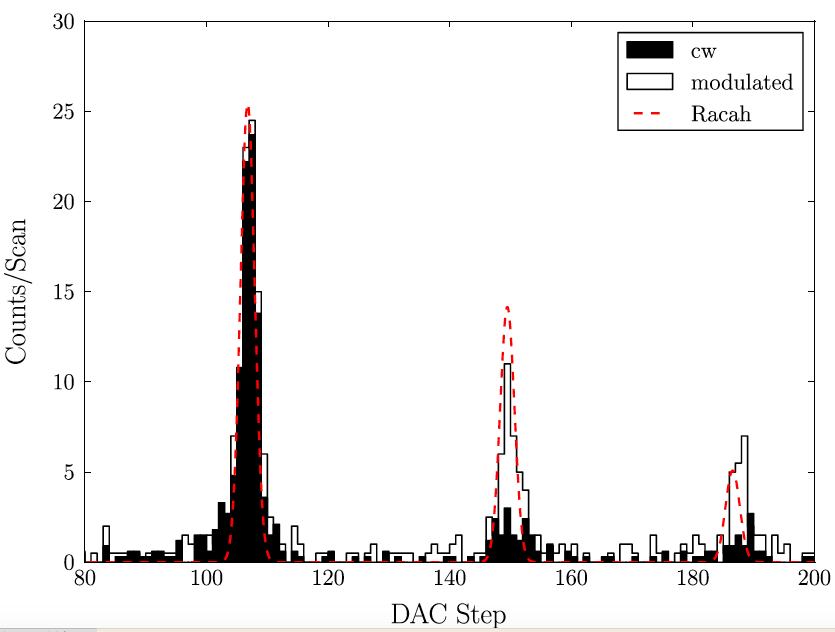
\includegraphics[width=\textwidth]{Graphics/francium.png}
\small
\caption{Demonstration of the effects of optical pumping on the relative peak heights for a hyperfine spectrum of Rb. The Racah intensities are shown in red, while the intensities measured for a continuous wave (cw) laser and a pulsed laser are shown in solid black and black lines, respectively. The cw measurements deviate significantly from the Racah intensities, while the pulsed measurements are closer to the expected intensities.\cite{CFBS}}
\label{OP_francium}
\end{figure}

To illustrate the effect of mechanisms of optical pumping, consider the following: A hyperfine system has two ground states, $\bf{F}_1$ and $\bf{F}_2$, as well as an excited state $\bf{F}_3$, as shown in Fig. \ref{toy_model}
\begin{figure}[h]
\begin{center}
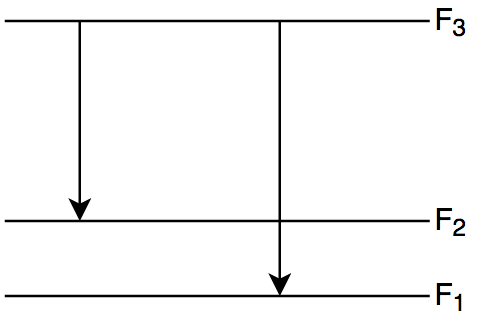
\includegraphics[width=\textwidth]{Graphics/Toy_model.png}
\small
\caption{Toy model of a hyperfine system with two ground states, $\bf{F}_1$ and $\bf{F}_2$, and a single excited state $\bf{F}_3$. If this system is exposed to a laser resonant with the $\bf{F}_2 \rightarrow \bf{F}_3$ transition, then as the atom goes through excitation and decay cycles, the chances of having an electron in $\bf{F}_2$ available for excitation decrease.}
\end{center}
\label{toy_model}
\end{figure}
When the atom is in the excited state, it has probability $P(\bf{F}_3 \rightarrow \bf{F}_2)$ of decaying to the $\bf{F}_2$ state, and probability $1-P(\bf{F}_3 \rightarrow \bf{F}_2)$ of decaying to the $\bf{F}_1$ state. If the atom is exposed to a laser resonant with the $\bf{F}_2 \rightarrow \bf{F}_3$ transition, what is the probability that after time $t$ the ground state of the atom is still $\bf{F}_2$? Say that the lifetime of the $\bf{F}_2 \rightarrow \bf{F}_3$ transition is $\tau$, and that the average time for a resonant photon to be absorbed is $t_{\mathrm{abs}}$. Then the number of excitation/decay cycles in time $t$, $N_{\mathrm{cycles}}$, is
\begin{equation}
N_{\mathrm{cycles}}=\frac{t}{\tau+t_{\mathrm{abs}}}.
\end{equation}
rounded down to the closest integer. If at any time, the atom decays to the $\bf{F}_1$ state, then it is no longer on resonance and the chances of a photon being absorbed are negligible. As such, the probability that the atom is in $\bf{F}_2$ after $N_{\mathrm{cycles}}$ is
\begin{equation}
P(\bf{F}_2) = P(\bf{F}_3 \rightarrow \bf{F}_2)^{N_{\mathrm{cycles}}}
\end{equation}
As $P(\bf{F}_3 \rightarrow \bf{F}_2) < 1$, then the chances of finding an electron in the $\bf{F}_2$ state decrease as $t$ increases. If, for example, one began measuring the number of resonant photons emitted after time $t$ for a collection of atoms with the above hyperfine structure, the number of photons measured would be reduced by a factor of $P(\bf{F}_2)$. This calculation is the basis for the method used in this work to measure the effect of optical pumping on the atoms being investigated at the CFBS, presented in the following section.

\section{Optical Pumping as a Modification to the Racah Intensities}
To evaluate the effects of optical pumping on a hyperfine spectrum collected at the CFBS experiment, the toy model presented above need only be expanded on. The important quantities are the time an atom interacts with the laser before entering the LCR, the time it takes for a resonant photon to be absorbed, the lifetimes of each excited state and the probability of an electron decaying to the ground state from which it originated. The computation of each of these quantities is presented in this section, after which they are combined to show how the Racah intensity for each transition must be modified to show the effects of optical pumping.

\subsection{Interaction Time}
The interaction time, $t_{\mathrm{int}}$ is the time that the atom will be possibly be interacting with the laser before entering the LCR. It's calculation is straightforward. If the distance between the CEC and the LCR is $d$, and the atoms are moving at a velocity $v$, then the interaction time is
\begin{equation}
t_{\mathrm{int}} = \frac{d}{v}
\end{equation}
While $d$ is a static quantity, $v$ changes depending on the frequency of the laser and the resonant frequency of the transition in question. As mentioned in Chapter \ref{Lspec}, the CFBS fixes the frequency of the laser and uses electrodes to alter the speed of the oncoming atoms, shifting the frequency observed by the atoms. Knowing the initial energy of the beam $E_b$ and the mass of the atoms $m_a$, the initial velocity of the atoms is 
\begin{equation}
v_{\mathrm{init}}=\sqrt{\frac{2E_b}{m_a}}
\end{equation}
If the resonant frequency of a transition is $f_{\mathrm{res}}$ and the frequency of the laser is $f_{\mathrm{las}}$, then the velocity at which the atom will observe $f_{\mathrm{res}}$, $v_{\mathrm{res}}$, is described by \cite{cmec}
\begin{equation}
f_{\mathrm{res}} = f_{\mathrm{las}} \sqrt{\frac{1+v_{\mathrm{res}}/c}{1-v_{\mathrm{res}}/c}}
\end{equation}
Rearranging yields the following expression for $v_{\mathrm{res}}$
\begin{equation}
v_{\mathrm{res}} = c \frac{(f_{\mathrm{res}}/f_{\mathrm{las}})^2-1}{(f_{\mathrm{res}}/f_{\mathrm{las}})^2+1}
\end{equation}
and
\begin{equation}
t_{\mathrm{int}} = \frac{d}{c} \frac{(f_{\mathrm{res}}/f_{\mathrm{las}})^2+1}{(f_{\mathrm{res}}/f_{\mathrm{las}})^2-1}
\end{equation}

\subsection{Absorption Time of a Resonant Photon}
For a chosen transition, what is the expected time, $t_{\mathrm{abs}}$ that passes before a resonant photon is absorbed by the atom, given a laser field of intensity $I$? This is simply the inverse of the scattering rate, as described in Eq. \ref{scatt_rate}, evaluated at resonance, i.e. $\delta = 0$
\begin{equation}
t_{\mathrm{abs}} = \left(\frac{s_0\gamma/2}{1+s_0}\right)^{-1}
\end{equation}

\subsection{Lifetime of an Excited State}
This quantity is already know. The inverse of Eq. \ref{gamma} gives the lifetime, $\tau$, of a particular transition
\begin{equation}
\tau = \frac{3\pi\epsilon_0\hbar c^3}{\omega^3\mu^2}
\end{equation}

\subsection{Time for Excitation/Decay Cycle}
Combining the results from the two above sections, the average time that it takes for an atom to go through an excitation/decay cycle, assuming that it returns to the ground state that it was in before excitation, $t_{\mathrm{cycle}}$, is
\begin{align}
t_{\mathrm{cycle}} =& t_{\mathrm{abs}}+ \tau\\
=& \left(\frac{s_0\gamma/2}{1+s_0}\right)^{-1} + \frac{3\pi\epsilon_0\hbar c^3}{\omega^3\mu^2}
\end{align}

\subsection{Probability of Returning to Original Ground State}
The probability of an atom decaying to the ground state from which it was excited is computed by comparing the decay rates of all possible transitions that share the same excited state as the transition in question, i.e., 
\begin{equation}
P(\mathrm{OGS}) = \frac{\gamma_{\mathrm{OGS}}}{\sum_{\mathrm{PT}}\gamma_{\mathrm{PT}}}
\end{equation}
where $P(\mathrm{OGS})$ is the probability of the atom returning to the original ground state, $\gamma_{\mathrm{OGS}}$ is the decay rate of the transition that results in the return to the original ground state and $\gamma_{\mathrm{PT}}$ is the decay rate of all possible transitions that share the same excited state as the transition in question.

\subsection{Probability of Reaching the LCR}
Finally, the probability of an atom reaching the LCR without changing its ground state is given by
\begin{equation}
P(\mathrm{OGS\ at\ LCR}) = \left(\frac{\gamma_{\mathrm{OGS}}}{\sum_{\mathrm{PT}}\gamma_{\mathrm{PT}}}\right)^{\frac{t_{\mathrm{int}}}{t_{\mathrm{cycle}}}}
\end{equation}
where $\frac{t_{\mathrm{int}}}{t_{\mathrm{cycle}}}$ is rounded down to the nearest integer, reflecting the fact the excitation/decay cycles are quantized events.

\section{Modification of the Racah Intensities}
Now that the probability of finding an atom in its original ground state when it reaches the LCR, the effects of optical pumping can be simulated through the modification of the Racah intensity for each transition. For a given transition $\bf{F}_e \rightarrow \bf{F}_g$ the modified Racah intensity, $I_{R_{\mathrm{mod}}}$, is 
\begin{align}
I_{R_{\mathrm{mod}}} =& P(\mathbf{F}_g\ \mathrm{at\ LCR})
(2F_e+1)(2F_g+1)
\left\lbrace
\mathrm{
\begin{matrix}
F_g & F_e & 1\\
J_e & J_g & \mathrm{I} 
\end{matrix}
}
\right\rbrace^2\\
=& \left(\frac{\gamma_{\mathrm{OGS}}}{\sum_{\mathrm{PT}}\gamma_{\mathrm{PT}}}\right)^{\frac{t_{\mathrm{int}}}{t_{\mathrm{cycle}}}}
(2F_e+1)(2F_g+1)
\left\lbrace
\mathrm{
\begin{matrix}
F_g & F_e & 1\\
J_e & J_g & \mathrm{I} 
\end{matrix}
}
\right\rbrace^2
\end{align}